\section{Langkah-Langkah Percobaan}
\begin{enumerate}
    \item Wireless Point to Point
    \begin{enumerate}
        \item Masuk winbox dan reset router. \newline
        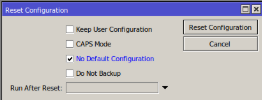
\includegraphics[scale=2]{P1/img/1.png}
        \item Aktifkan Interface Wireless Wlan 1 Masuk pada Menu 
        Wireless-> Wifi Interface -> Klik interface Wlan 1 dan 
        tekan tanda panah warna biru untuk enable Konfigurasikan 
        untuk Router A Sebagai ( setelah double Klik pada 
        interface wlan 1 masuk ke tab Wireless ) :
        \begin{itemize}
            \item Mode: Bridge
            \item SSID: PTP\_10
        \end{itemize}
        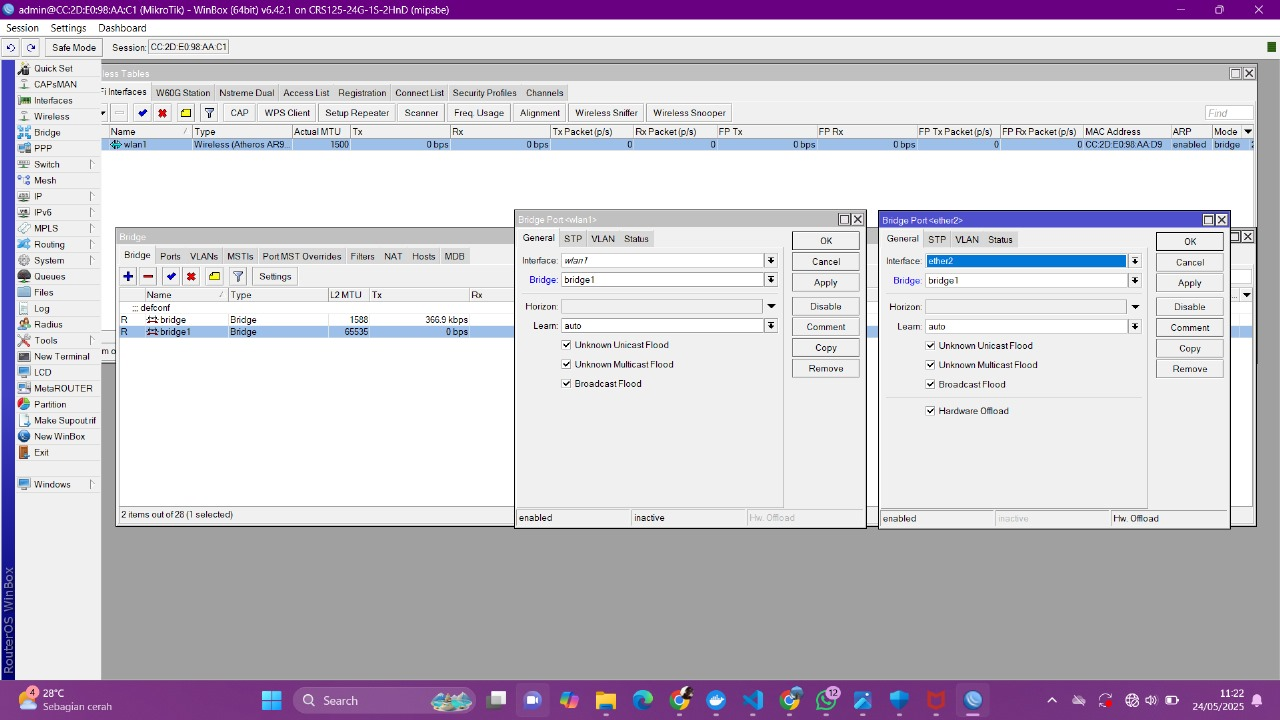
\includegraphics[scale=0.4]{P1/img/4.jpg} \newline
        Konfigurasikan untuk Router B Sebagai ( setelah double 
        Klik pada interface wlan 1 masuk ke tab Wireless ) :
        \begin{itemize}
            \item Mode: Station
            \item Setelah itu klik tombol scan dan pilih 
            interface menjadi wlan 1 lalu akan muncul berbagai 
            jaringan wifi cari nama wifi yang sesuai dengan 
            Router A lalu klik Connect.
        \end{itemize}
        \item Konfigurasi IP Address pada Wlan 1 Tambahkan IP 
        address pada Wlan 1 yang digunakan sebagai jalur 
        antar-router. Karena hanya ada dua perangkat yang 
        terhubung (router A dan router B),
        \begin{itemize}
            \item IP Wlan 1 Router A : 10.10.10.1/29
            \item IP Wlan 1 Router B : 10.10.10.2/29
        \end{itemize}
        \item Konfigurasi IP Address untuk Jaringan LAN (note 
        lakukan konfigurasi ini pada router A dan b) Tambahkan 
        IP address pada ether 2 yang digunakan untuk 
        menghubungkan Laptop dengan Router.
        \begin{itemize}
            \item IP ether 2 Router A : 192.168.20.1/24
            \item IP ether 2 Router B : 192.168.30.1/24 \newline
        \end{itemize}
        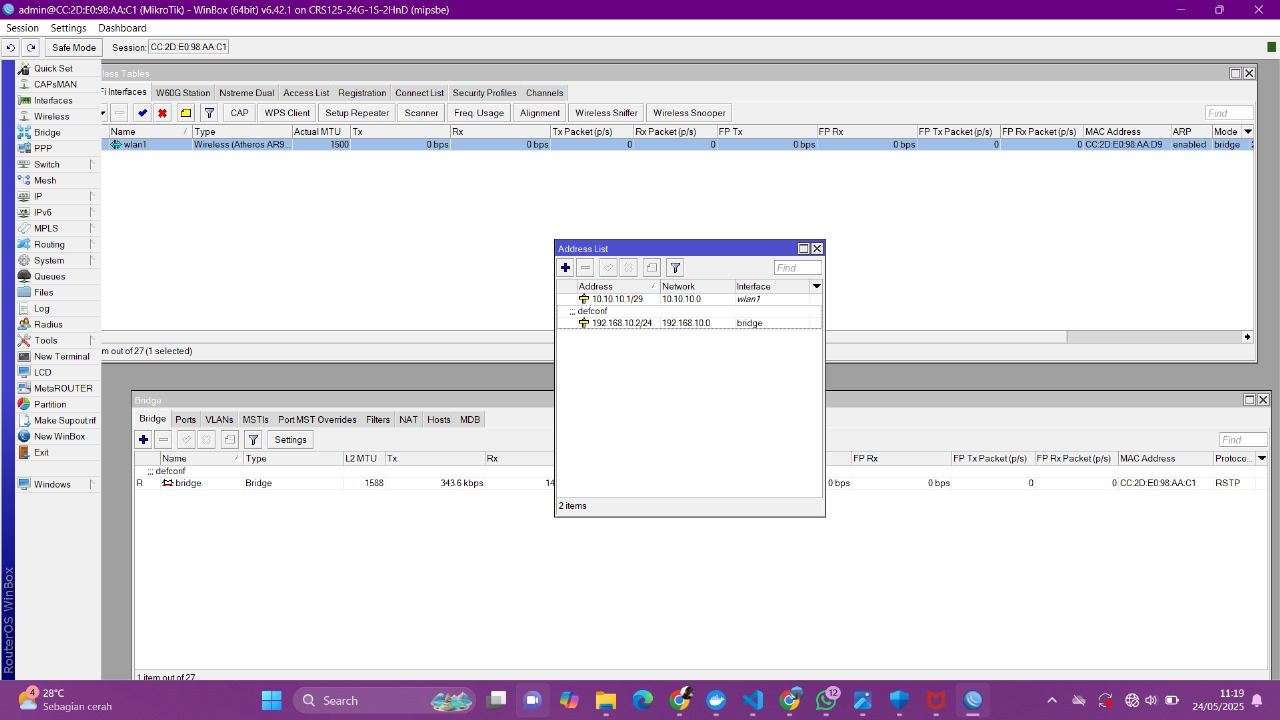
\includegraphics[scale=0.4]{P1/img/3.jpg} \newline
        \item Konfigurasi Routing Statis (note lakukan konfigurasi ini pada router A dan b) Setelah semua interface diberi IP, langkah selanjutnya adalah menambahkan rute secara manual. Masuk ke menu IPv4 → Routes, kemudian klik "+" untuk menambahkan routing. Pada Router A
        \begin{itemize}
            \item Dst. Address: 192.168.30.0/24
            \item Gateway: 10.10.10.2 Pada Router B
            \item Dst. Address: 192.168.20.0/24
            \item Gateway: 10.10.10.1
        \end{itemize}
        \item Test koneksi dengan melakukan ping antar router. \newline 
        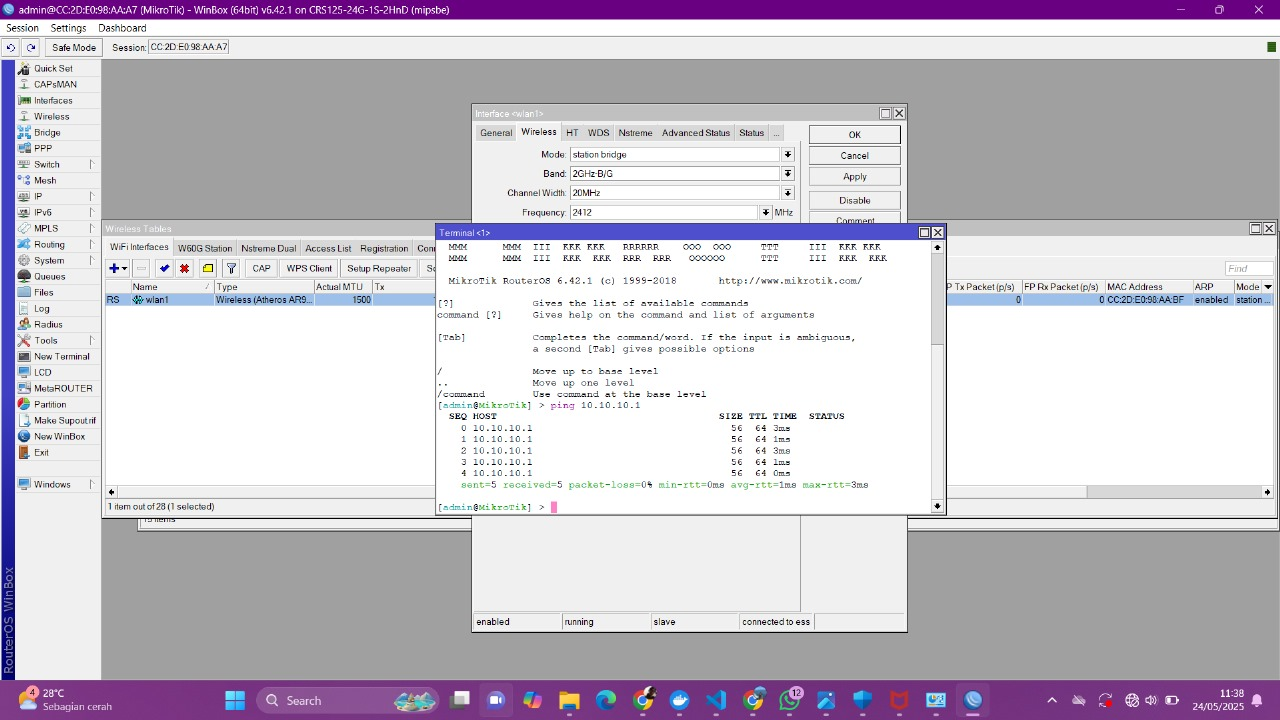
\includegraphics[scale=0.4]{P1/img/5.jpg} \newline
        \item Konfigurasi IP Adress di Laptop (note lakukan konfigurasi ini laptop yang terhubung pada router A dan b masing-masing) Karena ini masih menggunakan konfigurasi Static IP tambahkan IP address secara manual ke interface di laptop masing-masing bisa lewat Control Panel atau langsung di settings Windows, pastikan IP dan Gateway sudah benar sesuai Ether 2. Pada laptop yang terhubung ke Router A
        \begin{itemize}
            \item IP Address : 192.168.20.2
            \item Gateway : 192.168.20.1 (Router A)
            \item DNS : 8.8.8.8 \newline Pada laptop yang terhubung ke Router B
            \item IP Address: 192.168.30.2
            \item Gateway : 192.168.30.1 (Router B)
            \item DNS : 8.8.8.8
        \end{itemize}
        \item Test koneksi dengan melakukan ping antar laptop.
    \end{enumerate}
    \item Wireless Point to Multi Point
    \begin{enumerate}
        \item Masuk winbox dan reset router. \newline
        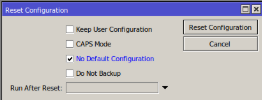
\includegraphics[scale=2]{P1/img/1.png}
        \item Aktifkan Interface Wireless Wlan 1 Masuk pada Menu Wireless-> Wifi Interface -> Klik interface Wlan 1 dan tekan tanda panah warna biru untuk enable Konfigurasikan untuk Router A Sebagai ( setelah double Klik pada interface wlan 1 masuk ke tab Wireless ) :
        \begin{itemize}
            \item Mode : Ap bridge
            \item SSID : PTMP\_10
        \end{itemize}
        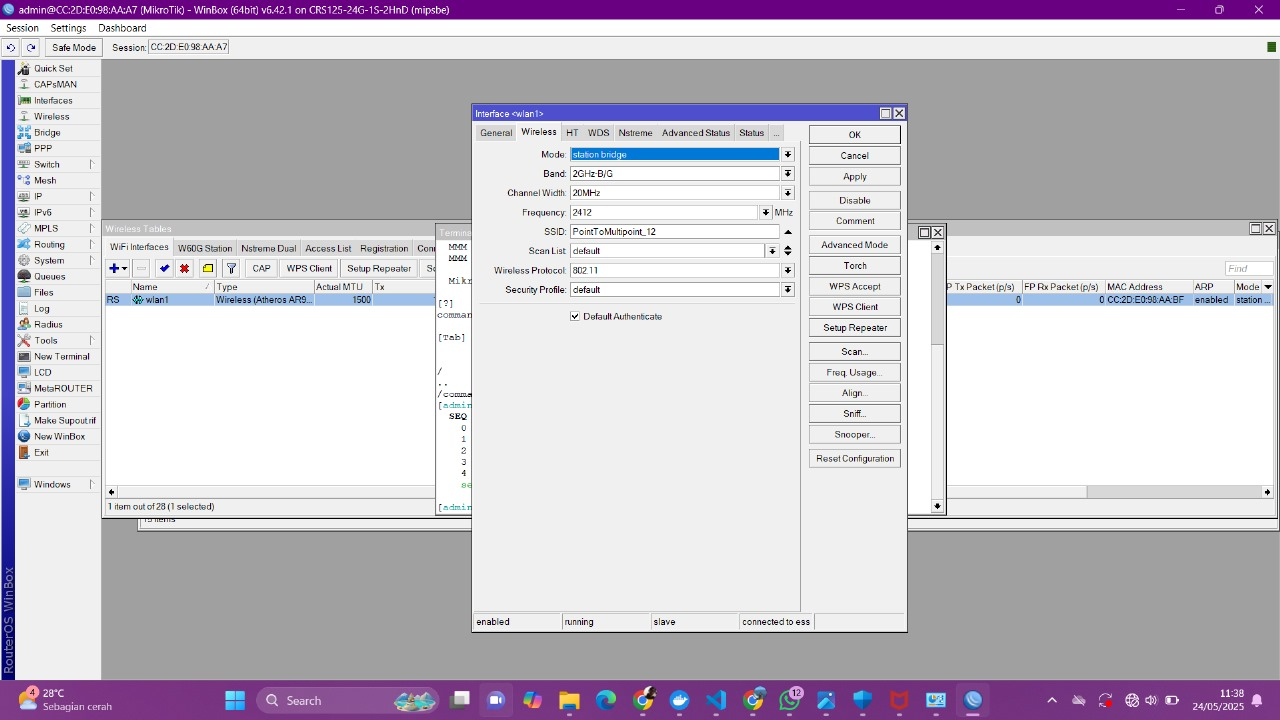
\includegraphics[scale=0.4]{P1/img/6.jpg} \newline
        \item Konfigurasikan untuk Router B Sebagai ( setelah double Klik pada interface wlan 1 masuk ke tab Wireless ) :
        \begin{itemize}
            \item Mode : Station Bridge
            \item Setelah itu klik tombol scan dan pilih interface menjadi wlan 1 lalu akan muncul berbagai jaringan wifi cari nama wifi yang sesuai dengan Router A lalu klik Connect.
        \end{itemize}
        \item Konfigurasi IP Address pada Wlan 1 Tambahkan IP address pada Wlan 1 yang digunakan sebagai jalur antar-router. Karena hanya ada dua perangkat yang terhubung (router A dan router B),
        \begin{itemize}
            \item IP Wlan 1 Router A : 10.10.10.1/29
            \item IP Wlan 1 Router B : 10.10.10.2/29
        \end{itemize}
        \item Konfigurasi IP Address untuk Jaringan LAN (note lakukan konfigurasi ini pada router A dan b) Tambahkan IP address pada ether 2 yang digunakan untuk menghubungkan Laptop dengan Router.
        \begin{itemize}
            \item IP ether 2 Router A : 192.168.20.1/24
            \item IP ether 2 Router B : 192.168.30.1/24
        \end{itemize}
        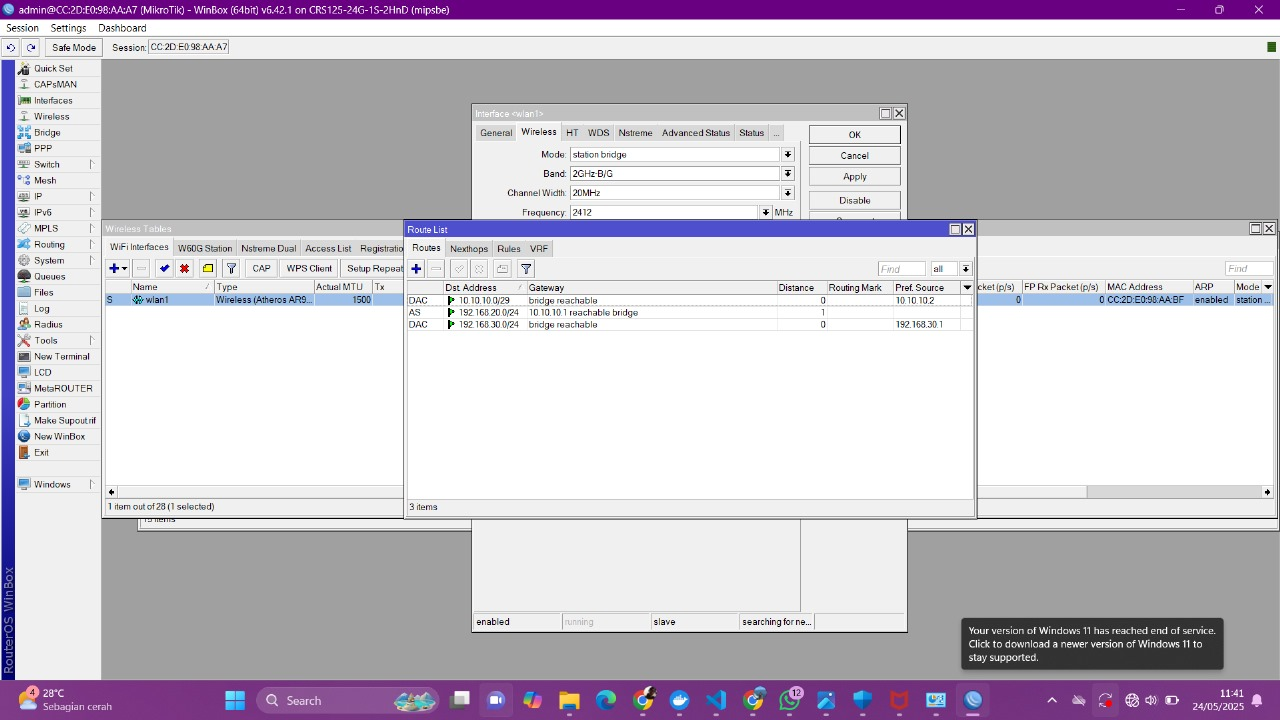
\includegraphics[scale=0.4]{P1/img/7.jpg} \newline
        \item Konfigurasi Routing Statis (note lakukan konfigurasi ini pada router A dan b) Setelah semua interface diberi IP, langkah selanjutnya adalah menambahkan rute secara manual. Masuk ke menu IPv4 → Routes, kemudian klik "+" untuk menambahkan routing. Pada Router A
        \begin{itemize}
            \item Dst. Address: 192.168.30.0/24
            \item Gateway: 10.10.10.2 Pada Router B
            \item Dst. Address: 192.168.20.0/24
            \item Gateway: 10.10.10.1
        \end{itemize}
        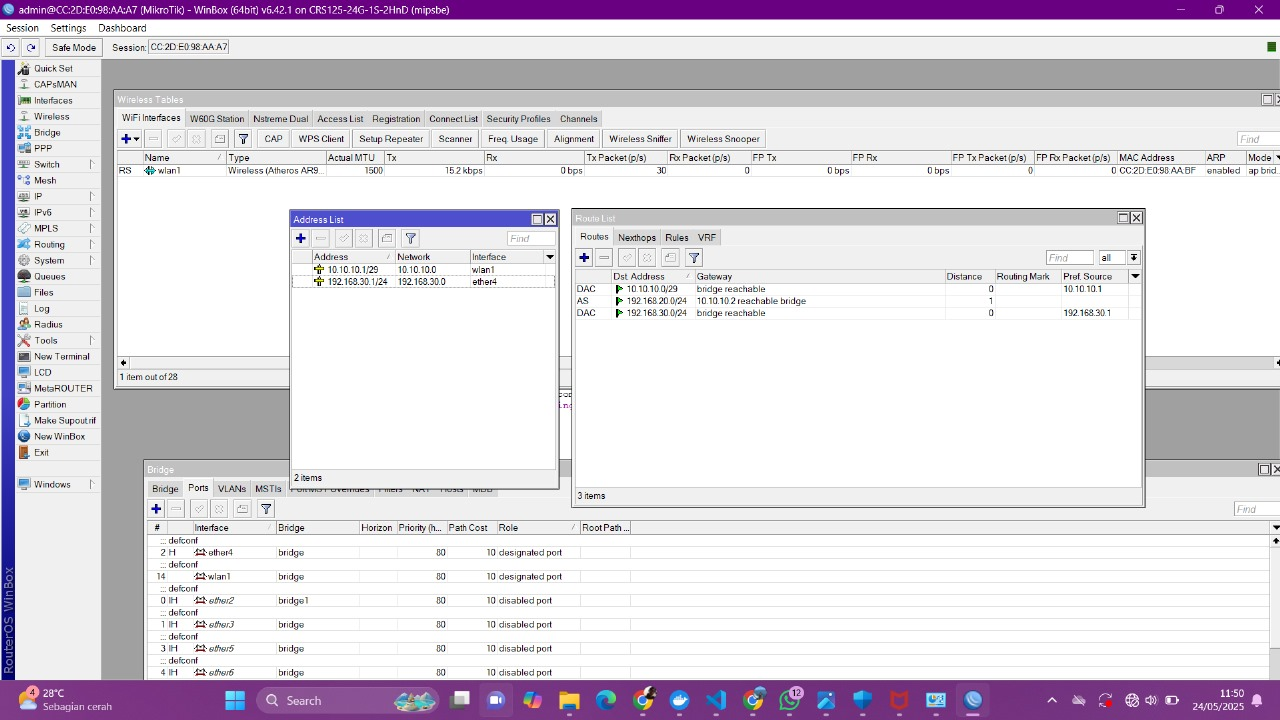
\includegraphics[scale=0.4]{P1/img/8.jpg} \newline
        \item Test koneksi dengan melakukan ping antar router.
        \item Konfigurasi IP Adress di Laptop (note lakukan konfigurasi ini laptop yang terhubung pada router A dan b masing-masing) Karena ini masih menggunakan konfigurasi Static IP tambahkan IP address secara manual ke interface di laptop masing-masing bisa lewat Control Panel atau langsung di settings Windows, pastikan IP dan Gateway sudah benar sesuai Ether 2. Pada laptop yang terhubung ke Router A
        \begin{itemize}
            \item IP Address : 192.168.20.2
            \item Gateway : 192.168.20.1 (Router A)
            \item DNS : 8.8.8.8 \newline Pada laptop yang terhubung ke Router B
            \item IP Address: 192.168.30.2
            \item Gateway : 192.168.30.1 (Router B)
            \item DNS : 8.8.8.8
        \end{itemize}
        \item Test koneksi dengan melakukan ping antar laptop.
    \end{enumerate}
    \item Wireless Bridge
    \begin{enumerate}
        \item Masuk winbox dan reset router. \newline
        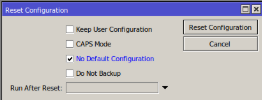
\includegraphics[scale=2]{P1/img/1.png}
        \item Aktifkan Interface Wireless Wlan 1 Masuk pada Menu Wireless-> Wifi Interface -> Klik interface Wlan 1 dan tekan tanda panah warna biru untuk enable Konfigurasikan untuk Router A Sebagai ( setelah double Klik pada interface wlan 1 masuk ke tab Wireless ) :
        \begin{itemize}
            \item Mode : Bridge
            \item SSID : WirelessBridge\_10
        \end{itemize}
        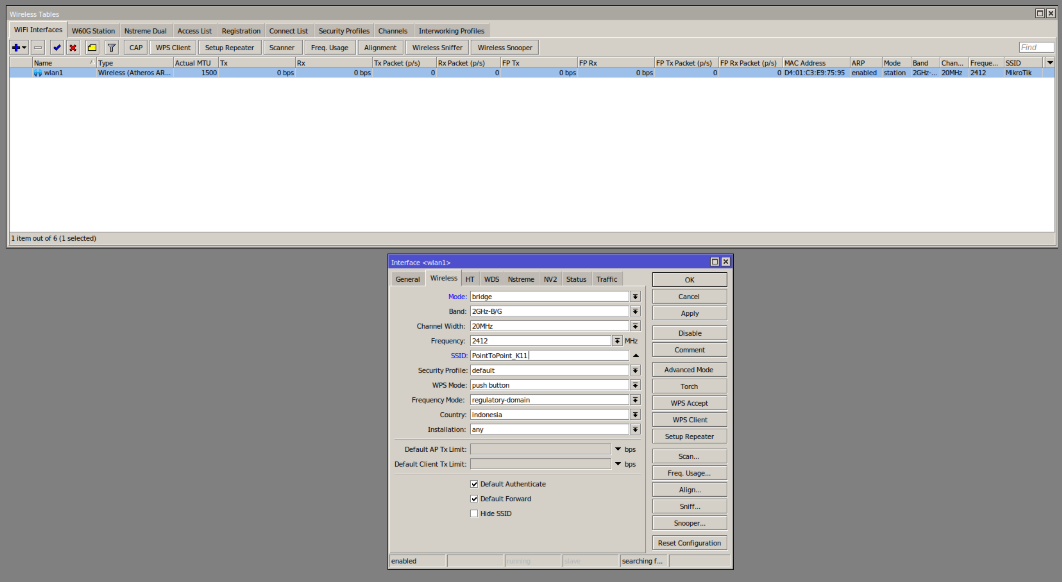
\includegraphics[scale=0.6]{P1/img/9.png} \newline
        Konfigurasikan untuk Router B Sebagai ( setelah double Klik pada interface wlan 1 masuk ke tab Wireless ) :
        \begin{itemize}
            \item Mode : Station Pseudobridge
            \item Setelah itu klik tombol scan dan pilih interface menjadi wlan 1 lalu akan muncul berbagai jaringan wifi cari nama wifi yang sesuai dengan Router A lalu klik Connect.
        \end{itemize}
        \item Konfigurasi IP Address pada Wlan 1 Tambahkan IP address pada Wlan 1 yang digunakan sebagai jalur antar-router. Karena hanya ada dua perangkat yang terhubung (router A dan router B),
        \begin{itemize}
            \item IP Wlan 1 Router A : 10.10.10.1/29
            \item IP Wlan 1 Router B : 10.10.10.2/29
        \end{itemize}
        \item Konfigurasi IP Address untuk Jaringan LAN (note lakukan konfigurasi ini pada router A dan b) Tambahkan IP address pada ether 2 yang digunakan untuk menghubungkan Laptop dengan Router.
        \begin{itemize}
            \item IP ether 2 Router A : 192.168.10.2/24
            \item IP ether 2 Router B : 192.168.10.3/24
        \end{itemize}
        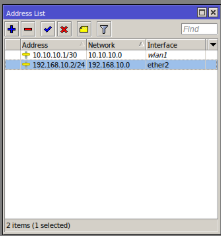
\includegraphics[scale=2]{P1/img/11.png} \newline
        \item Tambahkan bridge pada Router A dan B untuk menghubungkan wlan 1 dan ether 2 Router A :
        \begin{itemize}
            \item Masuk ke menu Bridge -> lalu tambah kan bridge dengan menekan tombol "+", lalu tambahkan untuk nama gunakan bridge1(atau yang lain)
            \item lalu masuk ke tab Port dan tambahkan :
            \item Interface Wlan 1 dan Ether 2 lalu gunakan bridge yang sudah di buat.
        \end{itemize}
        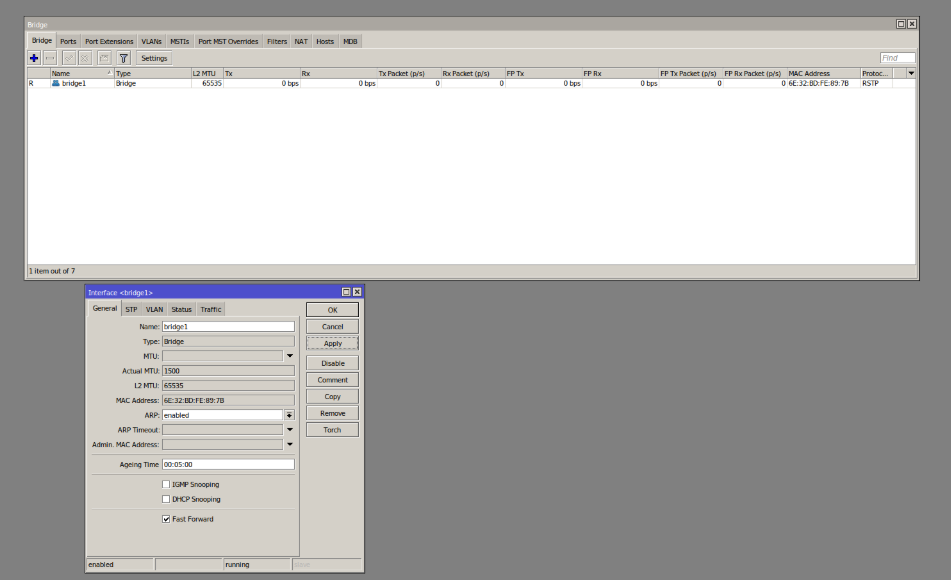
\includegraphics[scale=0.6]{P1/img/10.png} \newline
        \item Test koneksi dengan melakukan ping antar router.
        \item Konfigurasi IP Adress di Laptop (note lakukan konfigurasi ini laptop yang terhubung pada router A dan b masing-masing) Karena ini masih menggunakan konfigurasi Static IP tambahkan IP address secara manual ke interface di laptop masing-masing bisa lewat Control Panel atau langsung di settings Windows, pastikan IP dan Gateway sudah benar sesuai Ether 2. Pada laptop yang terhubung ke Router A
        \begin{itemize}
            \item IP Address : 192.168.10.5
            \item Gateway : 192.168.10.2 (Router A)
            \item DNS : 8.8.8.8 \newline Pada laptop yang terhubung ke Router B
            \item IP Address: 192.168.10.7
            \item Gateway : 192.168.10.3 (Router B)
            \item DNS : 8.8.8.8
        \end{itemize}
        \item Test koneksi dengan melakukan ping antar laptop.
    \end{enumerate}
\end{enumerate}
\section{Analisis Hasil Percobaan}
\begin{enumerate}
    \item Wireless Point to Point
    
    Pada uji coba jaringan Wireless Point to Point, dilakukan konfigurasi dengan menetapkan satu perangkat sebagai pemancar sinyal (bridge), sementara perangkat lainnya dikonfigurasi sebagai penerima (station). IP address pada interface wireless dan jaringan lokal diatur agar berada dalam satu subnet yang sama, sehingga kedua perangkat dapat saling terhubung melalui koneksi nirkabel tanpa menggunakan kabel. Hasil pengujian konektivitas menggunakan perintah ping menunjukkan respons yang sukses, menandakan bahwa koneksi wireless berjalan dengan baik dan stabil. Percobaan ini menunjukkan bagaimana gelombang radio dapat berfungsi sebagai pengganti kabel dalam menghubungkan dua lokasi secara langsung, sesuai prinsip dasar jaringan nirkabel yang fleksibel dan tidak terbatas oleh fisik kabel.
    \item Wireless Point to Multi Point
    
    Dalam pengujian jaringan Wireless Point to Multipoint, satu router dikonfigurasi sebagai titik pusat pemancar (dengan mode AP Bridge), sedangkan router lainnya berperan sebagai klien (dalam mode Station Bridge) yang menangkap sinyal tersebut. Proses koneksi dimulai dengan pemindaian SSID dan penyambungan klien ke titik akses berjalan lancar. Namun, efektivitas koneksi dipengaruhi oleh jarak dan penempatan antena. IP address dan routing statis disesuaikan agar kedua jaringan lokal dari masing-masing router dapat saling berkomunikasi, meskipun memiliki subnet berbeda. Hasil uji konektivitas ping menunjukkan bahwa koneksi antar perangkat berhasil dilakukan. Namun, performa jaringan dapat menurun apabila terdapat hambatan fisik atau jarak terlalu jauh, sehingga kestabilan koneksi perlu terus dipantau. Percobaan ini menunjukkan prinsip kerja jaringan multipoint serta tantangan riil yang mungkin dihadapi saat implementasi.

    Selama percobaan, terdapat hambatan seperti laptop yang gagal login ke Winbox sehingga harus diganti, serta router yang sering mati atau terputus dengan sendirinya, yang mengharuskan penggantian perangkat. Kendala-kendala tersebut merupakan faktor eksternal yang tidak dapat dihindari.
    \item Wireless Bridge
    
    Pada percobaan Wireless Bridge, dua jaringan lokal yang berbeda dihubungkan secara nirkabel melalui pengaturan mode bridge dan station pseudobridge. Dengan menggabungkan interface wireless dan ethernet ke dalam satu interface bridge, kedua jaringan dapat berinteraksi seolah-olah berada dalam satu jaringan fisik yang sama. Tujuan dari konfigurasi ini adalah agar perangkat di masing-masing jaringan bisa saling bertukar data tanpa hambatan, meskipun secara fisik mereka terpisah. Percobaan ini memperlihatkan bagaimana konsep wireless bridge memungkinkan integrasi dua jaringan lokal tanpa menggunakan kabel, namun tetap menjaga identitas jaringan masing-masing.

    Sayangnya, percobaan ini tidak sempat dilaksanakan karena keterbatasan waktu. Sebagian besar waktu habis akibat router yang terus-menerus logout otomatis dan proses login yang memakan waktu lama, sehingga pelaksanaan praktikum menjadi tidak memungkinkan.
\end{enumerate}
\section{Hasil Tugas Modul}
Simulasikan jaringan wireless antara tiga gedung:
\begin{enumerate}
    \item Gedung Pusat
    \item Gedung Lab
    \item Gedung Asrama (Hubungkan dua bagian dalam Gedung Asrama (Blok A dan Blok B) menggunakan Wireless Bridge Point-to-Point.)
\end{enumerate}

Berikut adalah hasil simulasi jaringan wireless antara tiga gedung:
\newline 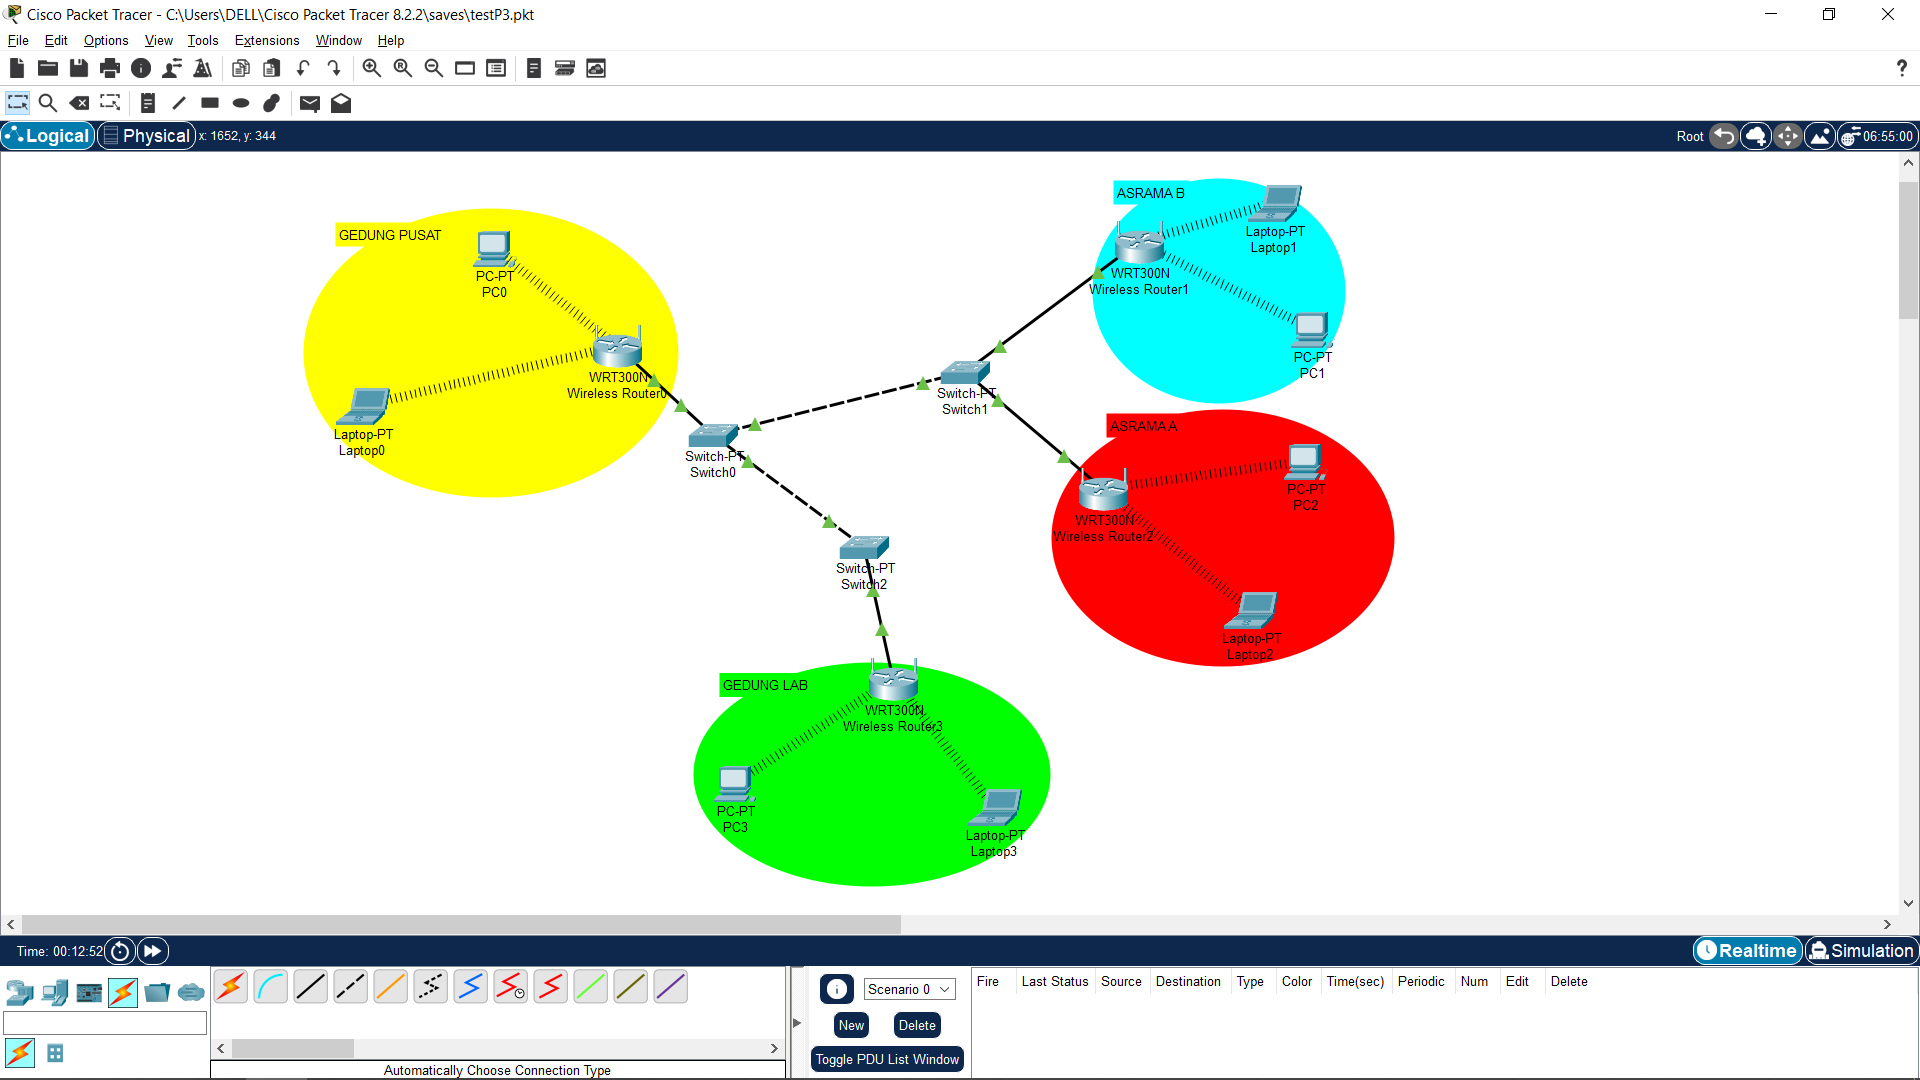
\includegraphics[scale=0.2]{P1/img/2.png}
\section{Kesimpulan}
Praktikum modul 3 ini mencakup rangkaian percobaan yang terdiri dari jaringan nirkabel Point to Point, Point to Multipoint, dan Wireless Bridge. Seluruh percobaan ini menekankan prinsip dasar komunikasi wireless, di mana gelombang radio digunakan sebagai alternatif dari kabel fisik dalam membangun koneksi jaringan. Pada skenario Point to Point, koneksi langsung antara dua perangkat berhasil diwujudkan secara stabil dengan menerapkan mode bridge dan station, serta pengaturan IP yang berada dalam satu subnet. Hal ini mencerminkan karakteristik jaringan wireless yang fleksibel dan tidak bergantung pada konektivitas kabel.

Selanjutnya, pada pengujian Point to Multipoint, terlihat bahwa satu perangkat pusat mampu menyebarkan sinyal ke banyak client sekaligus. Namun, tantangan seperti jarak dan hambatan fisik tetap menjadi faktor yang memengaruhi kualitas koneksi. Meskipun begitu, penetapan SSID yang konsisten serta konfigurasi routing statis memungkinkan perangkat dari jaringan yang berbeda subnet tetap dapat berkomunikasi dengan baik. Ini menggambarkan peran access point sebagai pusat distribusi sinyal dalam jaringan nirkabel.

Sementara itu, pada percobaan Wireless Bridge, dua jaringan lokal yang terpisah secara fisik berhasil dikoneksikan secara nirkabel melalui penggabungan interface wireless dan ethernet dalam satu bridge. Pendekatan ini memperlihatkan bagaimana bridge bertindak sebagai penghubung logis antara dua jaringan, memperluas jangkauan jaringan tanpa menghilangkan struktur segmentasi masing-masing jaringan.

Ketiga percobaan ini secara langsung mengimplementasikan teori dasar yang telah dipelajari, seperti mengaktifkan interface wireless, memilih mode operasi yang tepat (bridge, station, dan station pseudobridge), menetapkan SSID sebagai identitas jaringan, serta menentukan alamat IP dan subnet yang sesuai untuk mendukung komunikasi dan routing antar perangkat. Uji konektivitas dengan ping digunakan untuk memastikan jalur wireless telah terbentuk dengan andal. Secara keseluruhan, hasil praktikum ini membuktikan bahwa jaringan wireless dapat menjadi solusi yang efisien untuk berbagai topologi jaringan, memberikan kemudahan instalasi, mobilitas tinggi, dan kemampuan perluasan jaringan yang lebih fleksibel dibandingkan jaringan kabel tradisional.
\section{Lampiran}
\subsection{Dokumentasi saat praktikum}
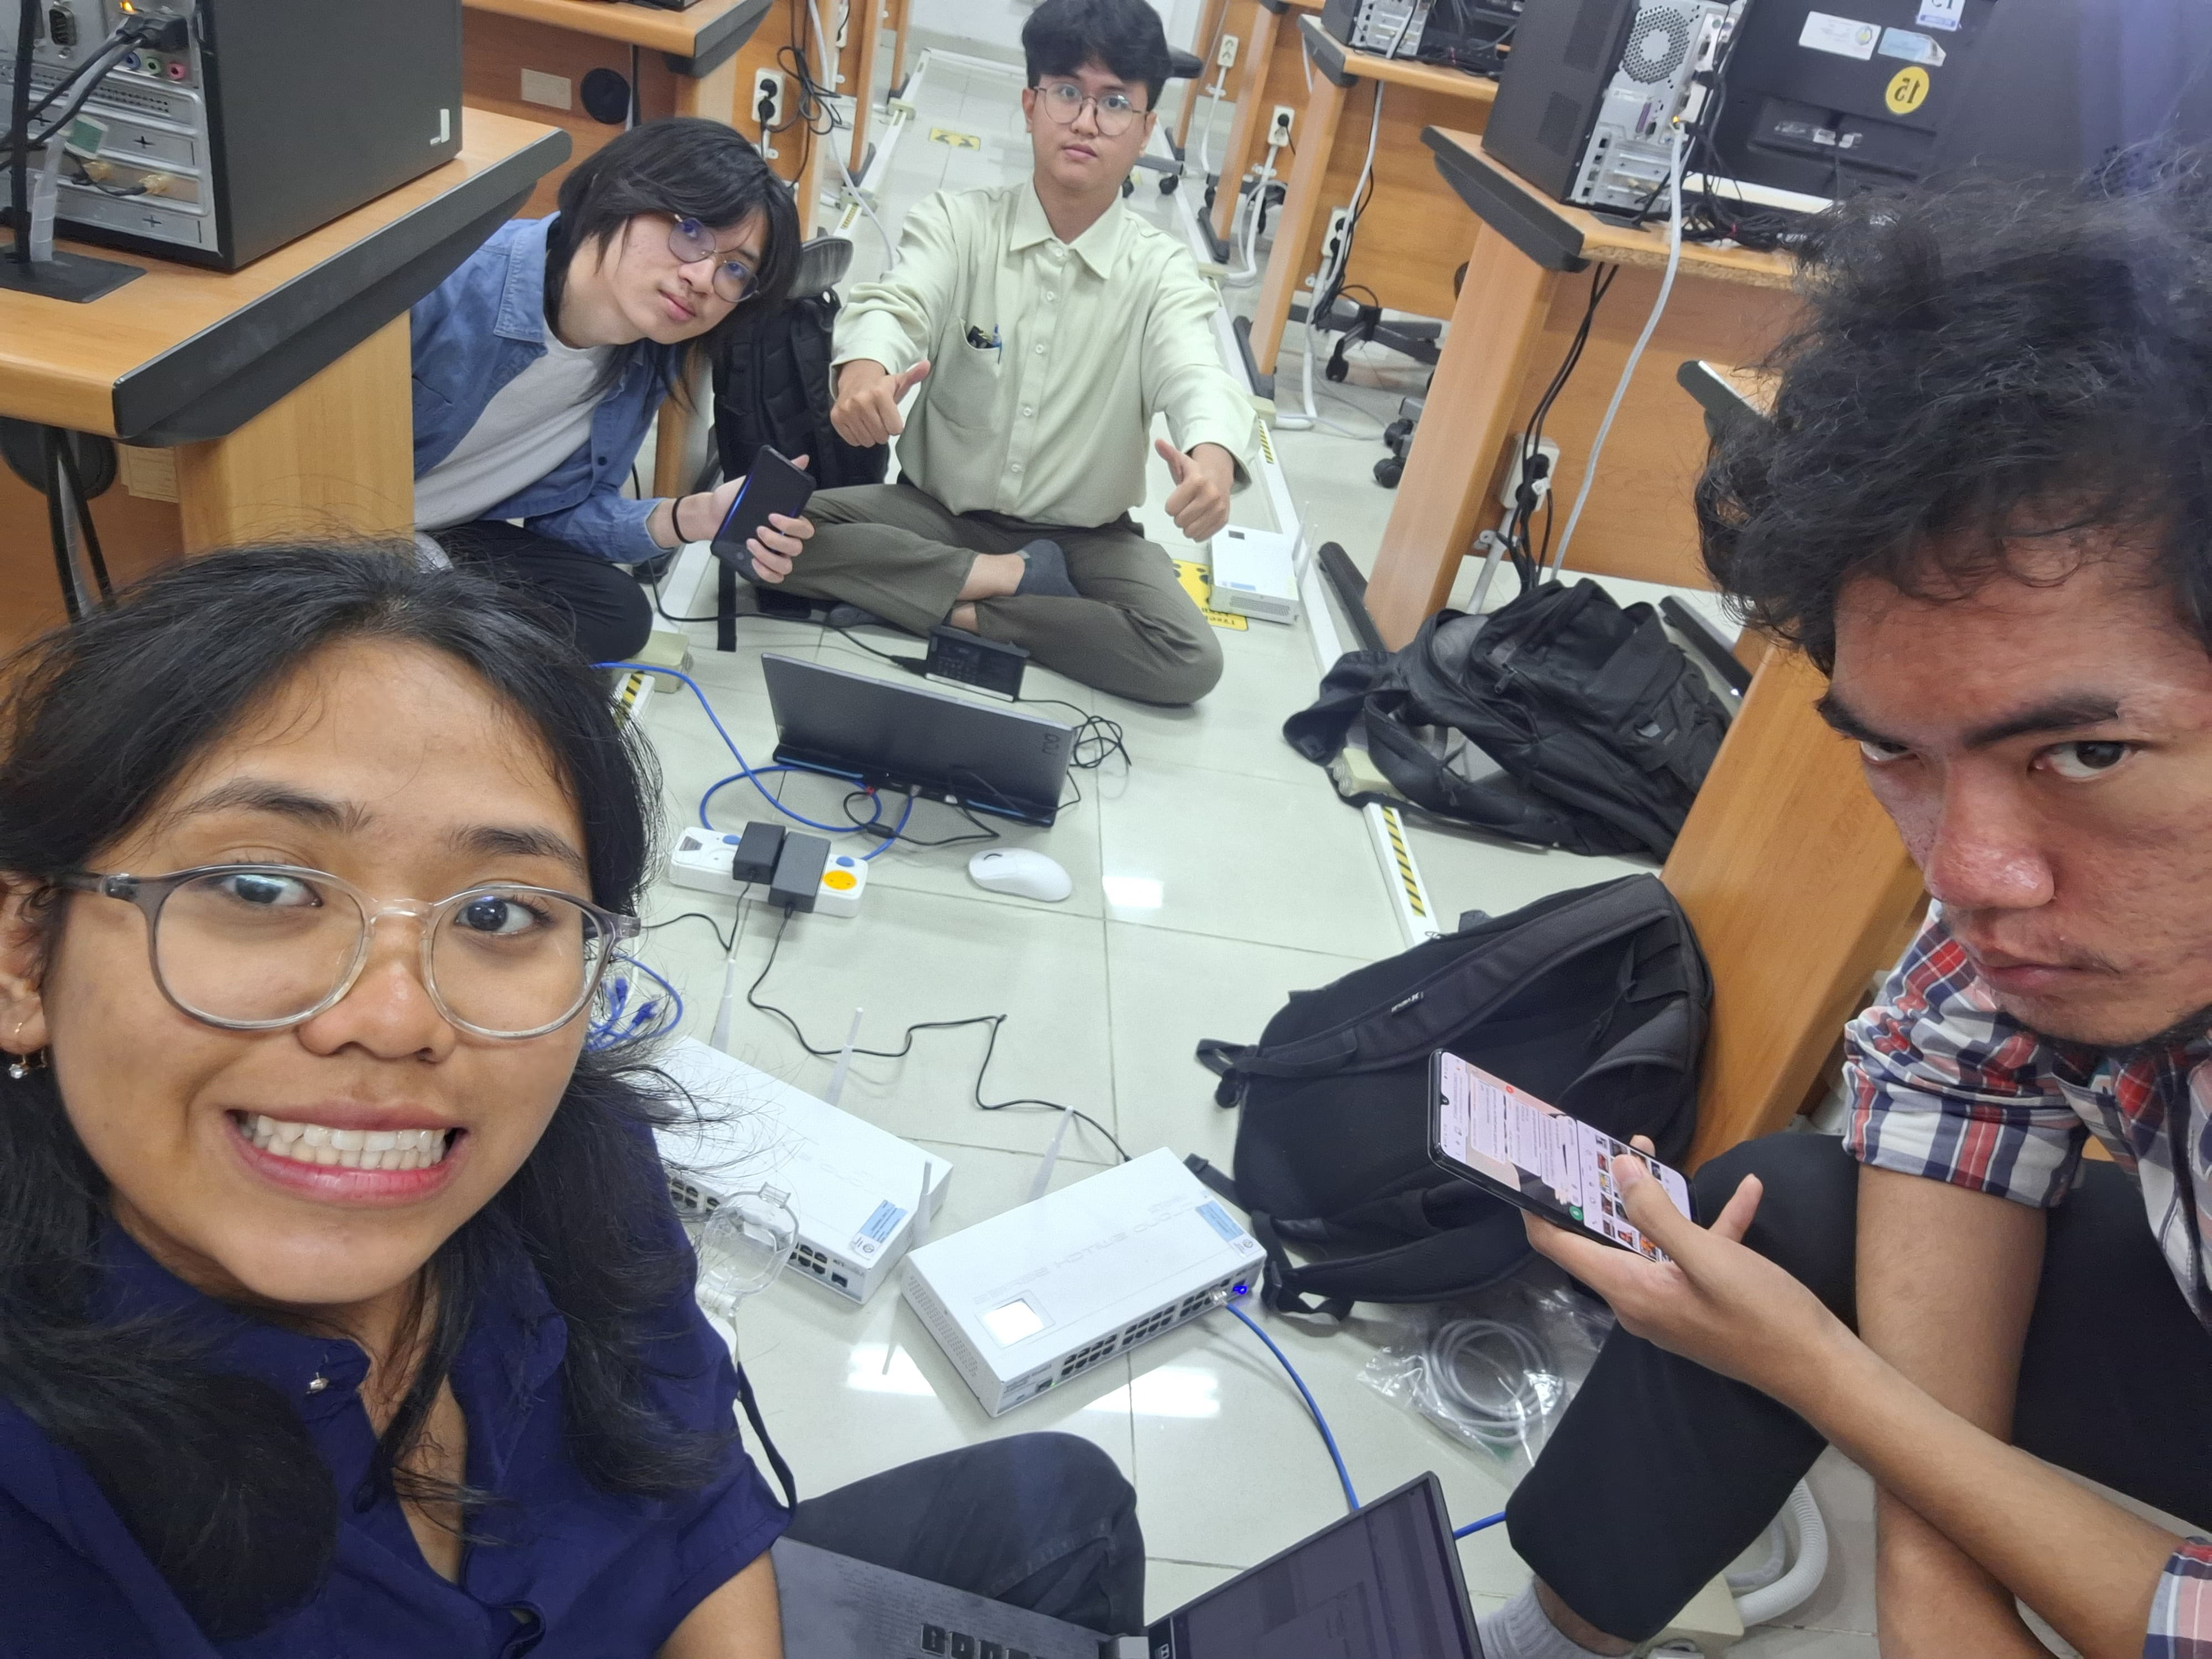
\includegraphics[scale=0.1]{P1/img/iniBuktinya.jpg}